\documentclass[final,3p,times,twocolumn]{elsarticle}

%% Use the option review to obtain double line spacing
%% \documentclass[preprint,review,12pt]{elsarticle}

%% Use the options 1p,twocolumn; 3p; 3p,twocolumn; 5p; or 5p,twocolumn
%% for a journal layout:
%% \documentclass[final,1p,times]{elsarticle}
%% \documentclass[final,1p,times,twocolumn]{elsarticle}
%% \documentclass[final,3p,times]{elsarticle}
%% \documentclass[final,3p,times,twocolumn]{elsarticle}
%% \documentclass[final,5p,times]{elsarticle}
%% \documentclass[final,5p,times,twocolumn]{elsarticle}

%% if you use PostScript figures in your article
%% use the graphics package for simple commands
%% \usepackage{graphics}
%% or use the graphicx package for more complicated commands
%% \usepackage{graphicx}
%% or use the epsfig package if you prefer to use the old commands
%% \usepackage{epsfig}

%% The amssymb package provides various useful mathematical symbols
\usepackage{amssymb}
%% The amsthm package provides extended theorem environments
%% \usepackage{amsthm}
%% The bm package lets you access bold symbols in math mode using the \boldsymbol command (useful to get bold greek letters).
\usepackage{bm}
%% The bbm (and also dsfont) package is contains the indicator function symbol \mathbbm{1}
\usepackage{bbm}
\usepackage{dsfont}
%% The amsmath package contains the split environment, letting you split equations into multiple lines.
%% See "https://www.sharelatex.com/learn/Aligning_equations_with_amsmath " for an explanation.
\usepackage{amsmath}
%% The lineno packages adds line numbers. Start line numbering with
%% \begin{linenumbers}, end it with \end{linenumbers}. Or switch it on
%% for the whole article with \linenumbers after \end{frontmatter}.
%% \usepackage{lineno}
%% The algorithm package defines the algorithm floating environment and the algpseudocode package is useful for constructing Pseudo code.
\usepackage{algorithm}
\usepackage{algpseudocode}
%% For making algorithms float
\usepackage{float}
\newfloat{algorithm}{t}{lop}
%% For drawing pictures inside latex
\usepackage{tikz}
%% For setting the 'DRAFT' watermark
%\usepackage{draftwatermark}
%\SetWatermarkText{DRAFT}
%\SetWatermarkScale{1}

%% Declaring \argmin and \argmax operators:
\DeclareMathOperator*{\argmin}{arg\,min}
\DeclareMathOperator*{\argmax}{arg\,max}
%% Declare trace operator \Tr:
\DeclareMathOperator*{\Tr}{Tr}
%% Declare pdf functions
\DeclareMathOperator*{\Dir}{Dir}
\DeclareMathOperator*{\Cat}{Cat}
%% shorthand for \boldsymbol
\let\bs\boldsymbol
%% Indicator symbol
\DeclareMathOperator*{\id}{\mathds{1}}
%% natbib.sty is loaded by default. However, natbib options can be
%% provided with \biboptions{...} command. Following options are
%% valid:

%%   round  -  round parentheses are used (default)
%%   square -  square brackets are used   [option]
%%   curly  -  curly braces are used      {option}
%%   angle  -  angle brackets are used    <option>
%%   semicolon  -  multiple citations separated by semi-colon
%%   colon  - same as semicolon, an earlier confusion
%%   comma  -  separated by comma
%%   numbers-  selects numerical citations
%%   super  -  numerical citations as superscripts
%%   sort   -  sorts multiple citations according to order in ref. list
%%   sort&compress   -  like sort, but also compresses numerical citations
%%   compress - compresses without sorting
%%
%% \biboptions{comma,round}

% \biboptions{}


\journal{MPhil in Scientific Computing}

\begin{document}

\begin{frontmatter}

%% Title, authors and addresses

%% use the tnoteref command within \title for footnotes;
%% use the tnotetext command for the associated footnote;
%% use the fnref command within \author or \address for footnotes;
%% use the fntext command for the associated footnote;
%% use the corref command within \author for corresponding author footnotes;
%% use the cortext command for the associated footnote;
%% use the ead command for the email address,
%% and the form \ead[url] for the home page:
%%
%% \title{Title\tnoteref{label1}}
%% \tnotetext[label1]{}
%% \author{Name\corref{cor1}\fnref{label2}}
%% \ead{email address}
%% \ead[url]{home page}
%% \fntext[label2]{}
%% \cortext[cor1]{}
%% \address{Address\fnref{label3}}
%% \fntext[label3]{}

\title{Implementation and Comparison of the $K$-Means algorithm and the Gaussian Mixture Model}

%% use optional labels to link authors explicitly to addresses:
%% \author[label1,label2]{<author name>}
%% \address[label1]{<address>}
%% \address[label2]{<address>}

\author{Brian Azizi}

\address{Cavendish Laboratory, Department of Physics, J J Thomson
  Avenue, Cambridge. CB3 0HE}

\begin{abstract}
Abstract.
\end{abstract}

\end{frontmatter}

%%
%% Start line numbering here if you want
%%
% \linenumbers

%% main text
\section{Introduction}
\label{sect:Intro}
The goal of \emph{clustering} is to discover structure in the data by identifying groups of similar data points. 
Clustering has found applications in biology (gene clustering), market research (market segmentation), grouping similar news (news clustering, eg Google News) and image segmentation (which has applications in medicine).

We begin by introducing a very simple clustering algorithm: $K$-Means. 
Then we make a small digression to discuss the related problem of density estimation (and outlier detection) which will lead to the Mixture of Gaussians model.


\section{$K$-Means Clustering}
In this section we introduce the \emph{$K$-Means algorithm} \cite{lloyd1982}.
It is one of the simplest and most intuitive approaches to clustering.
The algorithm requires only a single parameter to be set, namely the number of desired clusters $K$. 
It outputs a \emph{flat} and \emph{non-probabilistic} clustering of the data.

We start off by giving a general description of the method and stating the algorithm.
Following that, we look at its convergence properties and derive the formulas used in the algorithm.
We then discuss model selection in the context of $K$-means clustering and demonstrate the algorithm in a simple setting.
We finish the section with a brief discussion of extensions and generalizations of $K$-means.

\subsection{The $K$-Means algorithm}
Suppose we have data set $S = \{\bs x^{(1)},\dots,\bs x^{(N)}\}$ consisting of $N$ observations of the $D$ dimensional random variable $\bs X \in \mathbb{R}^D$.
We would like to partition the data into $K$ sets, where each set corresponds to a cluster.
For now, we assume that $K$ is given. In section \ref{sect:kmeans-ms}, we will discuss some common strategies for how $K$ can be set.

Each cluster $k$ is represented be a \emph{cluster centroids} $\bs\mu_k \in \mathbb{R}^D$.
We also need to introduce a latent variable $z^{(i)}$ for each data point $x^{(i)}$ that contains the \emph{cluster assignment} for sample $i$.
If $z^{(i)} = k$, then $x^{(i)}$ belongs to cluster $k$.

The $K$-Means algorithm starts by initializing the centroids $\boldsymbol \mu_k$.
Typically, this is done by randomly selecting $K$ distinct data points as the initial values for the centroid variables.

The algorithm then repeats the following two steps until convergence:
\begin{enumerate}
\item Assign each sample $x^{(i)}$ to the cluster represented by the centroid $\bs\mu_k$ that is closest to it.
\item Assign each cluster centroid $\bs\mu_k$ to the mean of all samples that currently belong to cluster $k$.
\end{enumerate}
The algorithm has converged once there are no more changes.
We have summarized the $K$-means algorithm in algorithm \ref{alg:kmeans}.

\begin{algorithm}
\caption{$K$-Means algorithm}
\label{alg:kmeans}
\begin{algorithmic}[1]
\State Initialize cluster centroids $\bs\mu_1,\dots,\bs\mu_K$
\Statex
\Repeat
\For{$i = 1,\dots,N$}
\State $z^{(i)} := \argmin_k ||\bs x^{(i)} - \bs\mu_k||^2$
\EndFor
\Statex
\For{$k = 1,\dots,K$}
\State $\bs\mu_k := \frac{\sum_{i=1}^N \id \{z^{(i)}\,=\,k\}\, \bs x^{(i)}}{\sum_{i=1}^N \id\{z^{(i)}\,=\,k\}}$
\EndFor
\Until{Convergence}
\Statex\State\Return{$z^{(1)}, \dots, z^{(N)}, \bs\mu_1, \dots, \bs\mu_K$}
\end{algorithmic}
\end{algorithm}


\subsection{Derivation and Convergence of $K$-Means}
\label{sect:kmeans-derivation}
In order to prove convergence of $K$-means, we define the \emph{distortion function} 
\begin{equation}
\label{eqn:distortion}
J(z^{(1)},\dots,z^{(N)},\bs\mu_1,\dots,\bs\mu_K) = \sum_{i=1}^N \sum_{k=1}^K \id\{z^{(i)}=k\}||\bs x^{(i)} - \bs \mu_k||^2
\end{equation}
The objective of $K$-Means clustering is equivalent to finding the parameters $z^{(i)} \in \{1,\dots,K\}$ and $\bs\mu_k\in\mathbb{R}^D$, for all $i$ and $k$, that minimize the distortion function $J$.

The $K$-means is obtained by applying the \emph{coordinate descent algorithm} to minimize the distortion function.
Coordinate descent is a simple optimization algorithm that can be used to find a local minimum of a multivariate function $F(\bs y)$.
It starts off by forming an initial guess $\bs y^{0}$ for the minimum $\bs y^*$. 
It then repeatedly cycles through each coordinate direction $y_j$ and minimizes $F$ along that direction.

In the case of the distortion function $J$, we only need to initialize the cluster centroids since the cluster assignments are independent of one another (the optimal value for $z^{(i)}$ tells us nothing about what $z^{(j)}$ should be).
We then minimize $J$ with respect to each $z^{(i)}$ keeping all other variables constant. 
If $K$ and $N$ are not too large, we can do this optimization by individually trying each value for $z^{(i)}$, i.e. by brute force.
The optimal value for $z^{(i)}$ is given by
\begin{equation}
\label{eqn:kmeans-E}
z^{(i)} = \argmin_k ||\bs x^{(i)} - \bs\mu_k||^2
\end{equation}
giving us the first inner loop of the $K$-means algorithm (lines 3-5 in algorithm \ref{alg:kmeans}).

Next, we minimize $J$ with respect to each cluster centroid $\bs\mu_k$ keeping all other variables constant.
We can do so by setting the gradient of $J$ with respect to $\bs\mu_k$ to zero:
\begin{equation}
\label{eqn:kmeans-M}
\begin{split}
\nabla_{\bs\mu_k} J &= \nabla_{\bs\mu_k} \sum_{i=1}^N\id\{z^{(i)}=k\}(\bs x^{(i)}-\bs\mu_k)^T(\bs x^{(i)}-\bs\mu_k)\\
&= -2 \sum_{i=1}^N\id\{z^{(i)}=k\}(\bs x^{(i)}-\bs\mu_k) = 0\\
\Rightarrow \bs\mu_k &= \frac{\sum_{i=1}^N\id\{z^{(i)} = k\}\,\bs x^{(i)}}{\sum_{i=1}^N\id\{z^{(i)}=k\}}
\end{split}
\end{equation}
This gives us the second inner loop of the algorithm (lines 6-8 in algorithm \ref{alg:kmeans}).
Furthermore, as already mentioned, (\ref{eqn:kmeans-M}) corresponds to setting $\bs \mu_k$ to the means of all samples $\bs x^{(i)}$ which currently assigned to cluster $k$.
\footnote{It is possible that $\sum_{i=1}^N\id\{z^{(i)}=k\} = 0$.
I.e. there is a possibility that a cluster becomes empty in the course of the algorithm.
If this happens, we can simply re-initialize the corresponding cluster centroid.
However, this may be an indication that we have set $K$ too large.}

One property of the coordinate descent algorithm is that each iteration is a (weak) improvement on the previous one.
This can be easily seen by noting that no update can make us worse off. 
So if the approximation to the solution at iteration $j$ is $\bs y^{(j)}$, then $F(\bs y^{(j)}) \geq F(\bs y^{(j+1)})$.
Hence, as long as the objective function is bounded below, the algorithm is guaranteed to converge to a local minimum.
Using the fact that $J \geq 0$, we have thus established convergence of the $K$-means algorithm.

Note, however, that we are only guaranteed to converge to a \emph{local} minimum.
In practice, this problem is dealt with by performing multiple runs of the entire $K$-Means algorithm.
We have to make sure that each run uses a different set of initial values for the the cluster centroids since, given an initialization, the $K$-means algorithm is completely deterministic.
We also need to record the final value of the distortion function $J$ after each run.
The overall output is then chosen to be the solution corresponding to the run for which the final value of $J$ was smallest.
Although this method does not guarantee convergence to the global optimum either, the resulting outcome is usually accepted to be at least ``good enough".

Convergence of the $K$-means algorithm was extensively studied by \cite{macqueen1967}.



\subsection{Model selection for $K$-Means Clustering}
\label{sect:kmeans-ms}
The only user-set parameter in the $K$-means algorithm is the number of clusters.
Therefore, model selection for $K$-means amounts to selecting the optimal value for $K$.

The standard model selection tool for $K$-means clustering is the so-called ``elbow method" (also referred to as the ``kink method").
We run the $K$-Means algorithm for a range of different values of $K$, say for $1 \leq K \leq K_{max}$, where $K_{max}$ is some preset maximum value for $K$.
For each run, the optimal value of the distortion function, $J^*_K$, is saved.
If necessary, perform multiple random initializations for each $K$ to avoid poor local optima.
Finally, we plot $J_K^*$ against $K$.

In some cases, it is possible to identify a distinct ``kink" in the curve at some $K^*$ (i.e. the curve has a noticable ``elbow").
If that is the case, it would be a reasonable choice to set $K$ to the value at which the kink occurs.

The intuition is that, if there is some true number of clusters $K^*$, we would expect a steep slope in the elbow curve for $K < K^*$.
If $K < K^*$, we are putting several clusters into the same group. 
Splitting the group into its constituent clusters should have a large effect on the distortion function.

If $K > K^*$, we have broken individual clusters into smaller groups.
Thus, we would expect only a small reduction in the distortion compared to $K^*$.

In practical applications, the optimal value for $K$ is often ambiguous.
In fact, a common behaviour of real-world data is that the number of clusters grows with the size of the data set.

Because of this, $K$ is usually chosen manually in practice.
In some applications, we domain-specific knowledge may give provide a reasonable value for $K$.

\subsection{Implementaion Details and Demonstration}


Figure \ref{fig:kmeans1} shows a result from running K-Means to convergence with $K = 3$.
\begin{figure}
\centering
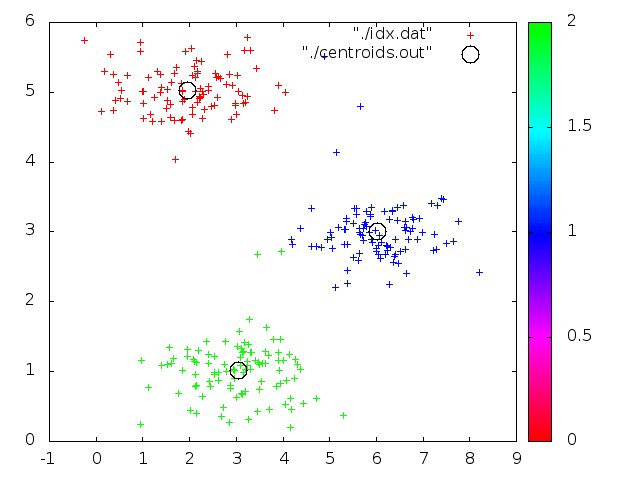
\includegraphics[width=3in]{kmeans1.png}
\caption{Result of running the K-Means algorithm on the toyclusters dataset with $K=3$}
\label{fig:kmeans1}
\end{figure}

However, it is possible for the K-Means algorithm to get stuck in local optima.
Figure \ref{fig:kmeans2} is the same as figure \ref{fig:kmeans1} but with a different initialization for the cluster centroids. 
\begin{figure}
\centering
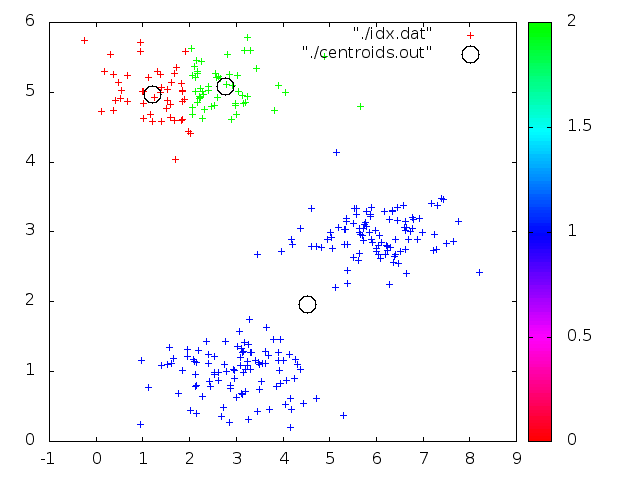
\includegraphics[width=3in]{kmeans2.png}
\caption{Local optimum of K-Means algorithm ($K=3$).}
\label{fig:kmeans2}
\end{figure}

\subsection{Extensions and Generalizations of $K$-Means}
We have described the K-Means algorithm using the squared Euclidean metric as a dissimilarity measure between data points.
It is possible to formulate the algorithm using a general dissimilarity metric $V(\boldsymbol x, \boldsymbol x')$.
In that case, the distortion function takes the form $J(\boldsymbol c, \boldsymbol \mu) = \sum_{i=1}^N V(\boldsymbol x^{(i)}, \boldsymbol \mu_{c^{(i)}})$.
The algorithm is then known as \emph{K-Medoids}.

For more information on K-Means clustering, see \cite{Bishop}.

\section{The Gaussian Mixture Model}
The Gaussian mixture model (GMM) (also known as mixtures of Gaussians) is the most widely used mixture model.
Before we explore its applications to clustering, let us first discuss the related problem of density estimation.
The goal of density estimation is to build the density $p(\boldsymbol x)$ of the random variable $\boldsymbol x \in \mathbb{R}^D$, given a set $\{\boldsymbol x^{(i)}\}_{i=1}^N$ of $N$ observations of $\boldsymbol x$.

Once we have formed the density $p(\boldsymbol x)$, we can apply the model to the problem of \emph{anomaly detection}.
Given a new observation $\boldsymbol x^{(N+1)}$, we flag it as an anomaly if $p(\boldsymbol x^{(N+1)}) < \epsilon$, where $\epsilon > 0$ is a pre-defined threshold.

The classical approach to density estimation is to assume $p(\boldsymbol x)$ belongs to some parametric family of distributions and to then infer the parameters from the data using tools such as \emph{maximum likelihood estimation}. 

\subsection{Modelling densities as mixtures of Gaussians}

What do we do if our data does not seem to come from any of the standard distributions (eg figure \ref{fig:gmm1}).
\begin{figure}
\centering
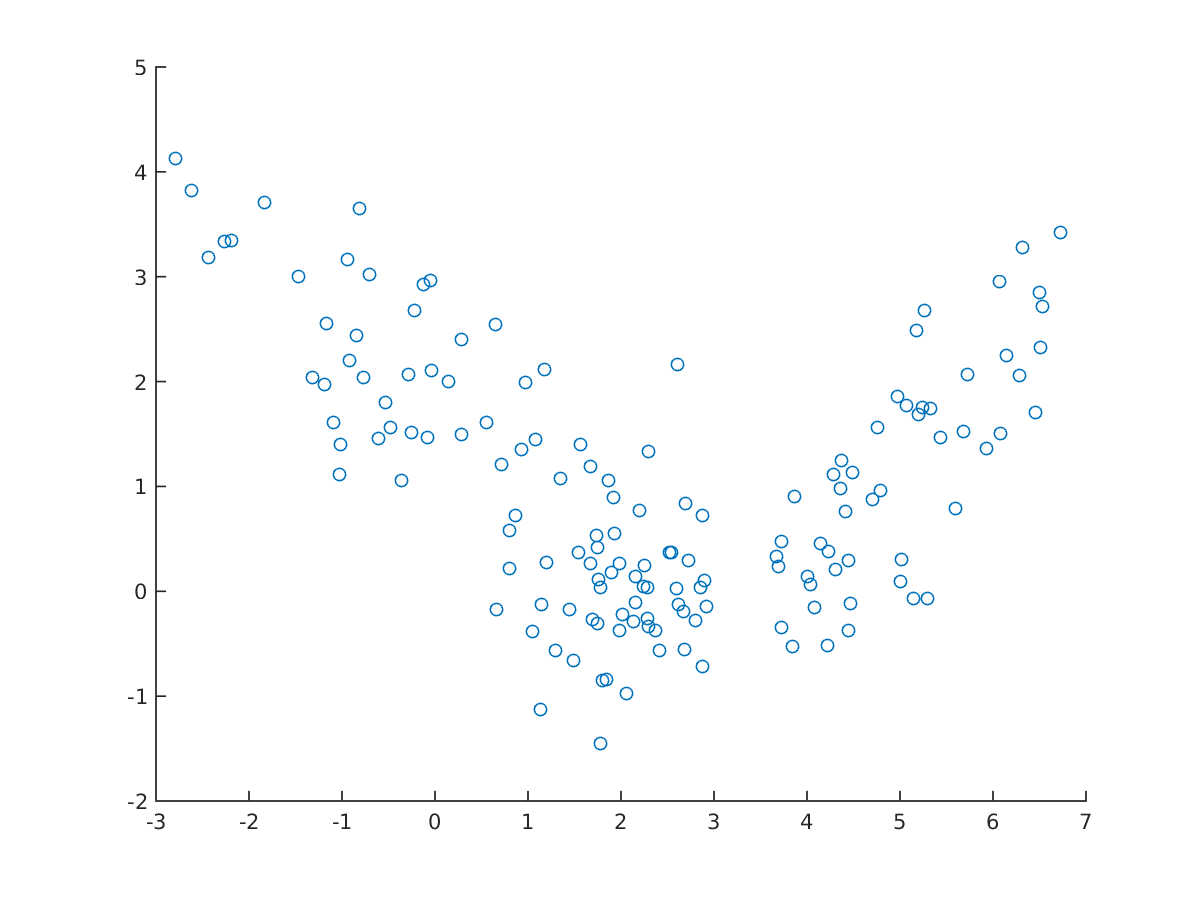
\includegraphics[width=3in]{gmm1.png}
%\caption{}
\label{fig:gmm1}
\end{figure}
One approach is to do non-parametric density estimation. A more straight forward strategy is to use a mixture model.
In the GMM, we assume that the data was generated from $K$ distinct Gaussian \emph{base distributions}. 
We do not know which Gaussian generated which data points, so we introduce the discrete latent variable $z^{(i)} \in \{1,2,\dots,K\}$ that tells us which cluster sample $\boldsymbol x^{(i)}$ belongs to.

We assume that 
\begin{equation}
z \sim Discrete(\,\boldsymbol \pi)
\label{eqnzdistro}
\end{equation}
\begin{equation}
\boldsymbol x \,|\, z \sim \mathcal{N}(\,\boldsymbol{\mu_z}, \boldsymbol \Sigma_z)
\label{eqn:x|z-distro}
\end{equation}
This means
\begin{equation}
p(z) = \pi_z, \qquad \pi_k > 0 \, \forall k \in \{1,\dots,K\}, \sum_{k=1}^K \pi_k = 1 
\end{equation}
\begin{equation}
\begin{split}
p(\boldsymbol x\,|\,z) &= \mathcal{N}(\boldsymbol x\,|\, \boldsymbol \mu_z, \boldsymbol \Sigma_z) \\
&= \frac{1}{\sqrt{2\pi\,|\Sigma_z|}}\exp(-\frac{1}{2}(\boldsymbol x - \boldsymbol \mu_z)^T\boldsymbol \Sigma_z^{-1} (\boldsymbol x - \boldsymbol \mu_z))\\
\end{split}
\end{equation}

From the sum rule and product rule of probability, we have
\begin{equation}
\begin{split}
p(\boldsymbol x) &= \sum_z p(\boldsymbol x, z) \\
&= \sum_z p(z)p(\boldsymbol x \,|\, z)\\
&= \sum_{k=1}^K \pi_k \mathcal{N}(\boldsymbol x\,|\,\boldsymbol \mu_k, \boldsymbol \Sigma_k)
\label{eqn:gmmdensity}
\end{split}
\end{equation}

\subsection{The EM algorithm for the GMM}
Given a training set $S$, how to we fit the model parameters $\{\pi_k, \boldsymbol \mu_k, \boldsymbol \Sigma_k; k=1,\dots,K\}$?
	If the labels $z^{(i)}$ were observed, we could formulate the likelihood of the data \footnote{In this case the model is equivalent to the quadratic discriminant analysis model used for classification} 
\begin{equation}
\mathcal{L}(\pi_k, \boldsymbol \mu_k, \boldsymbol \Sigma_k) = \prod_{i=1}^N p(\boldsymbol x^{(i)},z^{(i)}\,|\,\pi_k, \boldsymbol \mu_k, \boldsymbol \Sigma_k)
\label{eqn:LDAlikelihood}
\end{equation}
Maximising the likelihood would yield the following solutions for $k = 1,\dots,K$:
\begin{equation}
\begin{split}
\label{eqn:LDAstats}
&\pi_k = \frac{\sum_{i=1}^N \mathbbm{1}\{z^{(i)} = k\}}{N}\\
&\mu_k = \frac{\sum_{i=1}^N \mathbbm{1}\{z^{(i)} = k\} \boldsymbol{x}^{(i)}}{\sum_{i=1}^N \mathbbm{1}\{z^{(i)} = k\}}\\
&\Sigma_k = \frac{\sum_{i=1}^N \mathbbm{1}\{z^{(i)} = k\} (\boldsymbol{x}^{(i)} - \boldsymbol \mu_k)(\boldsymbol{x}^{(i)} - \boldsymbol \mu_k)^T}{\sum_{i=1}^N \mathbbm{1}\{z^{(i)} = k\}}\\
\end{split}
\end{equation}
(See the appendix for a derivation.)

In the unsupervised setting, we do not observe the values of $z^{(i)}$. 
Thus, the likelihood of our data now takes the form
\begin{equation}
	\mathcal{L}(\boldsymbol \pi, \boldsymbol \mu, \boldsymbol \Sigma) = \prod_{i=1}^N p(\boldsymbol x^{(i)}\,|\,\boldsymbol \pi, \boldsymbol \mu, \boldsymbol \Sigma)\\
\label{eqn:gmmLikelihood}
\end{equation}
Taking logs on both side and using equation \ref{eqn:gmmdensity}, we can formulate our objective function as
\begin{equation}
\begin{split}
\log\mathcal{L}(\boldsymbol \pi, \boldsymbol \mu, \boldsymbol \Sigma) &= \sum_{i=1}^N \log p(\boldsymbol x^{(i)}\,|\,\boldsymbol \pi \boldsymbol \mu, \boldsymbol \Sigma)\\
&= \sum_{i=1}^N \log \left(\sum_{k=1}^K \pi_k \mathcal{N}(\boldsymbol x^{(i)}\,|\, \boldsymbol \mu_k, \boldsymbol \Sigma_k)\right)\\
\end{split}
\label{eqn:gmmlogLikelihood}
\end{equation}

Maximising this objective function directly is problematic due to summation inside the logarithm term and there is, in fact, no known closed form solution.
Instead we use an iterative scheme in which we first formulate a ``guess" for the $z^{(i)}$ given our current parameter values and then find the optimal model parameters given our guess. 

Formally, we build the \emph{responsibility} that cluster $k$ takes for explaning sample $\boldsymbol x^{(i)}$, denoted $\gamma_k^{(i)}$.
This is defined to be the posterior probabibility that $z^{(i)} = k$:
\begin{equation}
\label{eqn:gmmresponsibility}
\begin{split}
y_k^{(i)} &= p(z^{(i)}=k\,|\,\boldsymbol x^{(i)}; \boldsymbol \pi, \boldsymbol \mu, \boldsymbol \Sigma)\\
	&= \frac{p(z^{(i)}=k;\boldsymbol \pi)p(\boldsymbol x^{(i)}\,|\,z^{(i)}=k;\boldsymbol \mu, \boldsymbol \Sigma)}
	{\sum_{j=1}^K p(z^{(i)}=j;\boldsymbol \pi)p(\boldsymbol x^{(i)}\,|\,z^{(i)}=j;\boldsymbol \mu, \boldsymbol \Sigma)}\\
	&= \frac{\pi_k\mathcal{N}(\boldsymbol x^{(i)}\,|\,\boldsymbol \mu_k, \boldsymbol \Sigma_k)}
	{\sum_{j=1}^K \pi_j\mathcal{N}(\boldsymbol x^{(i)}\,|\,\boldsymbol \mu_j, \boldsymbol \Sigma_j)}
\end{split}
\end{equation}

Once we have calculated the responsibilities, we can use them to update our model parameters.
\begin{equation}
\label{eqn:gmmstats}
\begin{split}
\pi_k &= \frac{\sum_{i=1}^N \gamma_k^{(i)}}{N}\\
\boldsymbol \mu_k &= \frac{\sum_{i=1}^N \gamma_k^{(i)} \boldsymbol x^{(i)}}{\sum_{i=1}^N \gamma_k^{(i)}}\\
\boldsymbol \Sigma_k &= \frac{\sum_{i=1}^N \gamma_k^{(i)}(\boldsymbol x^{(i)} - \boldsymbol \mu_k)(\boldsymbol x^{(i)} - \boldsymbol \mu_k)^T}{\sum_{i=1}^N \gamma_k^{(i)}}\\
\end{split}
\end{equation}
Note that we use the new value of $\boldsymbol \mu_k$ to calculate $\boldsymbol \Sigma_k$ in equation \ref{eqn:gmmstats}.
We iterate these two steps until convergence.
The typical convergence criterion is that changes in the loglikelihood are below some threshold.

Note the similarity with equation \ref{eqn:LDAstats}.
We have essentially replaced the indicators with \emph{soft weights} $\gamma_k^{(i)}$.
In the limit in which we observe $z^{(i)}$, we put all the probability mass on the observed value of $z^{(i)}$ and obtain $\gamma_k^{(i)} = \mathbbm{1}\{z^{(i)} = k\}$.

The algorithm above is a particular instance of the \emph{Expectation-Maximization (EM)} algorithm.
Equation \ref{eqn:gmmresponsibility} corresponds to the \emph{expectation step (E-step)} and equation \ref{eqn:gmmstats} corresponds to the \emph{maximization step (M-Step)} of the EM algorithm.
We will discuss the EM algorithm in more detail in the next section and also derive equations \ref{eqn:gmmresponsibility} and \ref{eqn:gmmstats}.
The pseudo-code for fitting the model parameters for the GMM can be found in algorithm \ref{alg:gmm}.

\begin{algorithm}
\caption{EM algorithm for GMM}
\label{alg:gmm}
\begin{algorithmic}[1]
\Procedure{EM for GMM}{$\boldsymbol X,K$}
\State{Randomly initialize $(\pi_k, \boldsymbol \mu_k, \boldsymbol \Sigma_k)$ for $k=1,\dots,K$}
\Repeat
\For{$i = 1:N$}\Comment{E-Step}
\State{$\gamma_k^{(i)} = \frac{\pi_k\mathcal{N}(\boldsymbol x^{(i)}\,|\,\boldsymbol \mu_k, \boldsymbol \Sigma_k)}
	{\sum_{j=1}^K \pi_j\mathcal{N}(\boldsymbol x^{(i)}\,|\,\boldsymbol \mu_j, \boldsymbol \Sigma_j)}$}
\EndFor
\For{$k = 1:K$}\Comment{M-Step}
\State{$\pi_k = \frac{\sum_{i=1}^N \gamma_k^{(i)}}{N}$}
\State{$\boldsymbol \mu_k = \frac{\sum_{i=1}^N \gamma_k^{(i)} \boldsymbol x^{(i)}}{\sum_{i=1}^N \gamma_k^{(i)}}$}
\State{$\boldsymbol \Sigma_k = \frac{\sum_{i=1}^N \gamma_k^{(i)}(\boldsymbol x^{(i)} - \boldsymbol \mu_k)(\boldsymbol x^{(i)} - \boldsymbol \mu_k)^T}{\sum_{i=1}^N \gamma_k^{(i)}}$}
\EndFor
\Until{Convergence}
\EndProcedure \\
	\Return{$\{(\gamma^{(1)}_k, \dots, \gamma^{(N)}_k, \pi_k, \boldsymbol \mu_k, \boldsymbol \Sigma_k), \quad k = 1,\dots,K\}$}
\end{algorithmic}
\end{algorithm}


\subsection{The EM algorithm: General setting}
The EM algorithm is powerful variational technique that is very popular in latent variable models.
In the general framework, we have a model for the joint distribution $p(x,z;\theta)$ (which is parameterized by $\theta$) but we only observe $x$.
Given a training data set $S=\{x^{(1)},\dots,x^{(N)}\}$, we would like to find the parameters $\theta$ that maximise the log likelihood of the data
\begin{equation}
\label{eqn:EMlikelihood}
\begin{split}
l(\theta) &= \sum_{i=1}^N \log p(x^{(i)};\theta)\\
&= \sum_{i=1}^N \log \sum_{z^{(i)}} p(x^{(i)},z^{(i)};\theta)
\end{split}
\end{equation}
The EM algorithm solves this problem in two steps.
In the expectation step, it forms a function that is a lower bound to $l(\theta)$ and that is tight at the current value of $\theta$.
In the maximization step, it finds $\theta$ that maximizes this lower bound.
This guarantees that we increase the value of $l(\theta)$ in each step (unless we are already at a maximum).

Let $Q_i(z^{(i)})$ be a probability measure on $z^{(i)}$, i.e. $Q_i(z^{(i)}) \geq 0$ and $\sum_{z^{(i)}} Q_i(z^{(i)}) = 1$. We can then express our objective function as
\begin{equation}
\begin{split}
l(\theta) &= \sum_{i=1}^N \log \sum_{z^{(i)}} p(x^{(i)},z^{(i)};\theta)\\
&= \sum_{i=1}^N \log \sum_{z^{(i)}} Q_i(z^{(i)}) \frac{p(x^{(i)},z^{(i)};\theta)}{Q_i(z^{(i)})}\\
&= \sum_{i=1}^N \log \mathbb{E}_{z^{(i)} \sim Q_i}\left[\frac{p(x^{(i)},z^{(i)};\theta)}{Q_i(z^{(i)})}\right]\\
\end{split}
\end{equation}

where we used the definition of the expectation operator. To proceed, we make use of \emph{Jensen's Inequality}: Let $X$ be a random variable and $f$ a convex function. Then
\begin{equation}
f(\mathbb{E}[X]) \leq \mathbb{E}[f(X)]
\label{eqn:jensen}
\end{equation}
Further, if $f$ is strictly convex, then 
\begin{equation}
\mathbb{E}[f(X)] = f(\mathbb{E}[X]) \iff p(X = E[X]) = 1
\label{eqn:jensentight}
\end{equation}
If $f$ is concave, then $-f$ is convex and thus the inequality is reversed.

By strict concavity of the log function, we thus have
\begin{equation}
\begin{split}
l(\theta) &=  \sum_{i=1}^N \log \mathbb{E}_{z^{(i)} \sim Q_i}\left[\frac{p(x^{(i)},z^{(i)};\theta)}{Q_i(z^{(i)})}\right]\\
&\geq \sum_{i=1}^N \mathbb{E}_{z^{(i)} \sim Q_i}\left[\log \frac{p(x^{(i)},z^{(i)};\theta)}{Q_i(z^{(i)})}\right]\\ 
&= \sum_{i=1}^N \sum_{z^{(i)}} Q_i(z^{(i)}) \log \frac{p(x^{(i)},z^{(i)};\theta)}{Q_i(z^{(i)})}\\ 
&= J(\theta,Q)
\end{split}
\end{equation}

where $Q=\{Q_1,\dots,Q_N\}$ and $J(\theta,Q)$ is a lower bound to $l(\theta)$ for all valid sets of probability measures $Q$.
We want to choose $Q_i$ such that the bound is tight at the current value of $\theta$.
Thus $p(x^{(i)},z^{(i)})/Q_i(z^{(i)})$ should be constant for all values of $z^{(i)}$. This implies that
\begin{equation}
\begin{split}
Q_i(z^{(i)}) &\propto p(x^{(i)},z^{(i)};\theta)\\
\Rightarrow Q_i(z^{(i)}) &= \frac{p(x^{(i)},z^{(i)};\theta)}{\sum_{z^{(i)}}p(x^{(i)},z^{(i)};\theta)}\\
&= \frac{p(x^{(i)},z^{(i)};\theta)}{p(x^{(i)};\theta)}\\
&= p(z^{(i)}\,|\,x^{(i)};\theta);
\end{split}
\end{equation}
where the second line follows from the normalization constraint on $Q_i$, the third line from the sum rule of probability and the fourth line from the definition of conditional probabilities.

This completes the E-Step of the EM algorithm.
In the M-Step, we maximise $J(\theta,Q) = \sum_{i=1}^N \sum_{z^{(i)}} Q_i(z^{(i)}) \log \left(p(x^{(i)},z^{(i)};\theta)/Q_i(z^{(i)})\right)$ with respect to $\theta$, keeping $Q_i = p(z^{(i)}\,|\,x^{(i)};\theta)$ fixed.\footnote{Thus, the EM algorithm is analogous to coordinate ascent on $J(\theta,Q)$}.
See algorithm \ref{alg:EM} for a summary.

\begin{algorithm}
\caption{EM algorithm}
\label{alg:EM}
\begin{algorithmic}[1]
\Procedure{EM}{$\boldsymbol X,K$}
\State{Randomly initialize $\theta$}
\Repeat
\State{E-Step:}
\For{$i = 1:N$}
\State{Set $Q_i(z^{(i)}) = p(z^{(i)}\,|\,x^{(i)};\theta)$}
\EndFor
\State{M-Step:}
\State{$\theta = \argmax_\theta \sum_{i=1}^N \sum_{z^{(i)}} Q_i(z^{(i)}) \log \frac{p(x^{(i)},z^{(i)};\theta)}{Q_i(z^{(i)})}$}
\Until{Convergence}
\EndProcedure \\
\Return{$(\theta,\{(z^{(1)}, \dots, z^{(N)}\})$}
\end{algorithmic}
\end{algorithm}

In the Gaussian mixture model, for the E-step we have
\begin{equation}
\label{eqn:gmmE}
\begin{split}
Q_i(z^{(i)} = k) &= p(z^{(i)} = k\,|\,\boldsymbol x^{(i)}; \boldsymbol \pi, \boldsymbol \mu, \boldsymbol \Sigma)\\
&= p(z^{(i)}=k\,|\,\boldsymbol x^{(i)}; \boldsymbol \pi, \boldsymbol \mu, \boldsymbol \Sigma)\\
&= \frac{p(z^{(i)}=k;\boldsymbol \pi)p(\boldsymbol x^{(i)}\,|\,z^{(i)}=k;\boldsymbol \mu, \boldsymbol \Sigma)}
{\sum_{j=1}^K p(z^{(i)}=j;\boldsymbol \pi)p(\boldsymbol x^{(i)}\,|\,z^{(i)}=j;\boldsymbol \mu, \boldsymbol \Sigma)}\\
&= \frac{\pi_k\mathcal{N}(\boldsymbol x^{(i)}\,|\,\boldsymbol \mu_k, \boldsymbol \Sigma_k)}
{\sum_{j=1}^K \pi_j\mathcal{N}(\boldsymbol x^{(i)}\,|\,\boldsymbol \mu_j, \boldsymbol \Sigma_j)} = \gamma_k^{(i)}
\end{split}
\end{equation}

While in the M-Step we want to find $\pi_k$, $\boldsymbol \mu_k$ and $\boldsymbol \Sigma_k$ that maximize
\begin{equation}
\label{eqn:gmmM1}
\begin{split}
J(\boldsymbol \pi, \boldsymbol \mu, \boldsymbol \Sigma, \boldsymbol \gamma) &= \sum_{i=1}^N\sum_{z^{(i)}} Q_i(z^{(i)}) \log \frac{p(\boldsymbol x^{(i)},z^{(i)};\boldsymbol \pi, \boldsymbol \mu, \boldsymbol \Sigma)}{Q_i(z^{(i)})}\\
&= \sum_{i=1}^N \sum_{k=1}^K \gamma_k^{(i)} \log \frac{\pi_j \mathcal{N}(\boldsymbol x^{(i)} \,|\, \boldsymbol \mu_k, \boldsymbol \Sigma_k)}{\gamma_k^{(i)}}\\
\end{split}
\end{equation}
Setting the derivative with respect to $\boldsymbol \mu_k$ equal to zero gives
\begin{equation}
\begin{split}
\label{eqn:gmmMu}
\nabla_{\boldsymbol \mu_k} J &= \sum_{i=1}^N -\frac{1}{2}\gamma_k^{(i)} \nabla_{\boldsymbol \mu_k} (\boldsymbol x^{(i)} - \boldsymbol \mu_k)^T \boldsymbol \Sigma^{-1}(\boldsymbol x^{(i)} - \boldsymbol \mu_k)\\
&= \sum_{i=1}^N -\frac{1}{2}\gamma_k^{(i)}(\boldsymbol \Sigma_k^{-1} + \boldsymbol \Sigma_k^{-T})(\boldsymbol \mu_k - \boldsymbol x^{(i)})\\
&= \sum_{i=1}^N\gamma_k^{(i)} \boldsymbol \Sigma^{-1} (\boldsymbol x^{(i)} - \boldsymbol \mu_k) = 0\\
\Rightarrow \boldsymbol \mu_k &= \frac{\sum_{i=1}^N\gamma_k^{(i)} \boldsymbol x^{(i)}}{\sum_{i=1}^N \gamma_k^{(i)}}
\end{split}
\end{equation}
To find the optimal $\boldsymbol \Sigma_k$, we note that this equivalent to finding $\boldsymbol \Sigma_k^{-1}$ that maximizes $J$:
\begin{equation}
\label{eqn:gmmSigma}
\begin{split}
\nabla_{\boldsymbol \Sigma_k^{-1}} J &= \sum_{i=1}^N \gamma_k^{(i)}(\frac{1}{2}\nabla_{\boldsymbol \Sigma_k^{-1}}(\log |\boldsymbol \Sigma_k^{-1}| - (\boldsymbol x^{(i)} - \boldsymbol \mu_k)^T \boldsymbol \Sigma_k^{-1}(\boldsymbol x^{(i)} - \boldsymbol \mu_k))\\
&= \sum_{i=1}^N \gamma_k^{(i)} \frac{1}{2}(\boldsymbol \Sigma_k - (\boldsymbol x^{(i)} - \boldsymbol \mu_k)(\boldsymbol x^{(i)} - \boldsymbol \mu_k)^T) = 0\\
\Rightarrow \boldsymbol \Sigma_k &= \frac{\sum_{i=1}^N \gamma_k^{(i)}(\boldsymbol x^{(i)} - \boldsymbol \mu_k)(\boldsymbol x^{(i)} - \boldsymbol \mu_k)^T}{\sum_{i=1}^N \gamma_k^{(i)}}
\end{split}
\end{equation}
The mixing coefficients $\boldsymbol \pi$ must satisfy the constraint $\sum_{k=1}^K \pi_k = 1$.
We use the method of Lagrange multipliers to perform the constrained optimization.
Let $\lambda > 0$ denote the Lagrange multiplier.
To find the optimal coefficients $\pi_k$, we set the derivative of $(J(\boldsymbol \pi, \boldsymbol \mu, \boldsymbol \Sigma, \boldsymbol \gamma) + \lambda(1-\sum_{k=1}^K \pi_k))$ with respect to $\pi_k$ to zero.
\begin{equation}
\label{eqn:gmmPi1}
\begin{split}
\frac{\partial}{\partial \pi_k}(J + \lambda(1 - \sum_{k=1}^K \pi_k)) &= \sum_{i=1}^N\gamma_k^{(i)} \frac{\partial}{\partial \pi_k} \log \pi_k - \lambda\\
&= \sum_{i=1}^N \frac{\gamma_k^{(i)}}{\pi_k} - \lambda = 0\\
\Rightarrow \pi_k = \frac{\sum_{i=1}^N\gamma_k^{(i)}}{\lambda}
\end{split}
\end{equation}
Taking the sum over $k$ on both sides gives
\begin{equation}
\label{eqn:gmmPi2}
\begin{split}
1 &= \frac{\sum_{i=1}^N \sum_{k=1}^K \gamma_k^{(i)}}{\lambda}\\
\Rightarrow \lambda &= \sum_{i=1}^N \sum_{k=1}^K \gamma_k^{(i)}\\
&= \sum_{i=1}^N 1 = N
\end{split}
\end{equation}
Since $\sum_{k=1}^K \gamma_k^{(i)} = \sum_{k=1}^K p(z^{(i)} = k\,|\,\boldsymbol x^{(i)}) = 1$.
Thus,
\begin{equation}
\pi_k = \frac{\sum_{i=1}^N \gamma_k^{(i)}}{N}.
\label{eqn:gmmPi3}
\end{equation}

\subsection{Model Selection in the Gaussian mixture model}
It is possible for the EM algorithm to get stuck in local optima.
The approach of dealing with this problem is analogous to the one used in the K-Means algorithm:
We perform multiple runs of the EM algorithm with different random initializations of the GMM parameters. We then pick the result for which the log likelihood was greatest.

In order to choose $K$, we may again employ the ``elbow method'', by plotting the negative log likelihood against $K$.
Another popular approach is the use information theoretic model selection criteria such as the \emph{Akaike Information Criterion (AIC)}, the \emph{Bayesian Information Criterion (BIC)} or the \emph{Kullbeck-Leibler Information Criterion (KLIC)}.
It is also possible to embed the GMM in a Bayesian framework by putting prior probabilities on our model parameters.
For instance, we could put a Gaussian-Inverse-Wishart prior on the cluster means and covariances and a Dirichlet prior on the mixing coefficients.
These priors are conjugate to our likelihood function and thus lead to fast computation of the posterior probabilities of the parameters. \emph{(CHECK THIS)}.
\emph{COMMENT: how is this used for model selection?}

\subsection{KMeans as limit of GMM}
We can derive the K-Means algorithm as a special case of the EM algorithm for the Gaussian Mixture Model.
Let is fix $\pi_k = 1/K$ and $\boldsymbol \Sigma_k = \sigma^2 \boldsymbol I_D$ for all values of $k$.
Further, let us approximate the responsibilities by delta functions
\begin{equation}
\label{eqn:gmmdelta}
\gamma_k^{(i)} = \mathbbm{1}\{z^{(i)} = k^*\}
\end{equation}
where
\begin{equation}
k^* = \argmax_k p(z^{(i)} = k\,|\,\boldsymbol x^{(i)},\boldsymbol \pi, \boldsymbol \mu, \boldsymbol \Sigma)
\end{equation}
is the MAP estimate of $z^{(i)}$.
Due to the spherical covariance matrix, $k^*$ will be simply equal to the identity of the currently closest cluster centroid to $\boldsymbol x^{(i)}$. This completes the E-step.

In the M-Step, we only need to update the cluster means $\boldsymbol \mu_k$.
Using our approximations for $\gamma_k^{(i)}$, the GMM update formula for $\boldsymbol \mu_k$ reduces to the one we used in the K-Means algorithm, i.e. the empirical mean of all data points currently assigned to cluster $k$.

For more info, see \cite{Bishop} and \cite{Murphy}.


\section*{Acknowledgements}
Here I acknowledge the assistance of my supervisor, my industrial sponsor,
and the effects of caffine on my ability to produce this report on time.

%% The Appendices part is started with the command \appendix;
%% appendix sections are then done as normal sections
\appendix

\section{Derivation of GMM with known cluster identities}
\label{app:gmm}

%% References
%%
%% Following citation commands can be used in the body text:
%% Usage of \cite is as follows:
%%   \cite{key}         ==>>  [#]
%%   \cite[chap. 2]{key} ==>> [#, chap. 2]
%%

%% References with bibTeX database:
\section*{Bibliography}
\bibliographystyle{elsarticle-num}
\bibliography{references.bib}

%% Authors are advised to submit their bibtex database files. They are
%% requested to list a bibtex style file in the manuscript if they do
%% not want to use elsarticle-num.bst.

%% References without bibTeX database:

% \begin{thebibliography}{00}

%% \bibitem must have the following form:
%%   \bibitem{key}...
%%

% \bibitem{}

% \end{thebibliography}


\end{document}

%%
%% End of file `mini.tex'.